\documentclass[1p]{elsarticle_modified}
%\bibliographystyle{elsarticle-num}

%\usepackage[colorlinks]{hyperref}
%\usepackage{abbrmath_seonhwa} %\Abb, \Ascr, \Acal ,\Abf, \Afrak
\usepackage{amsfonts}
\usepackage{amssymb}
\usepackage{amsmath}
\usepackage{amsthm}
\usepackage{scalefnt}
\usepackage{amsbsy}
\usepackage{kotex}
\usepackage{caption}
\usepackage{subfig}
\usepackage{color}
\usepackage{graphicx}
\usepackage{xcolor} %% white, black, red, green, blue, cyan, magenta, yellow
\usepackage{float}
\usepackage{setspace}
\usepackage{hyperref}

\usepackage{tikz}
\usetikzlibrary{arrows}

\usepackage{multirow}
\usepackage{array} % fixed length table
\usepackage{hhline}

%%%%%%%%%%%%%%%%%%%%%
\makeatletter
\renewcommand*\env@matrix[1][\arraystretch]{%
	\edef\arraystretch{#1}%
	\hskip -\arraycolsep
	\let\@ifnextchar\new@ifnextchar
	\array{*\c@MaxMatrixCols c}}
\makeatother %https://tex.stackexchange.com/questions/14071/how-can-i-increase-the-line-spacing-in-a-matrix
%%%%%%%%%%%%%%%

\usepackage[normalem]{ulem}

\newcommand{\msout}[1]{\ifmmode\text{\sout{\ensuremath{#1}}}\else\sout{#1}\fi}
%SOURCE: \msout is \stkout macro in https://tex.stackexchange.com/questions/20609/strikeout-in-math-mode

\newcommand{\cancel}[1]{
	\ifmmode
	{\color{red}\msout{#1}}
	\else
	{\color{red}\sout{#1}}
	\fi
}

\newcommand{\add}[1]{
	{\color{blue}\uwave{#1}}
}

\newcommand{\replace}[2]{
	\ifmmode
	{\color{red}\msout{#1}}{\color{blue}\uwave{#2}}
	\else
	{\color{red}\sout{#1}}{\color{blue}\uwave{#2}}
	\fi
}

\newcommand{\Sol}{\mathcal{S}} %segment
\newcommand{\D}{D} %diagram
\newcommand{\A}{\mathcal{A}} %arc


%%%%%%%%%%%%%%%%%%%%%%%%%%%%%5 test

\def\sl{\operatorname{\textup{SL}}(2,\Cbb)}
\def\psl{\operatorname{\textup{PSL}}(2,\Cbb)}
\def\quan{\mkern 1mu \triangleright \mkern 1mu}

\theoremstyle{definition}
\newtheorem{thm}{Theorem}[section]
\newtheorem{prop}[thm]{Proposition}
\newtheorem{lem}[thm]{Lemma}
\newtheorem{ques}[thm]{Question}
\newtheorem{cor}[thm]{Corollary}
\newtheorem{defn}[thm]{Definition}
\newtheorem{exam}[thm]{Example}
\newtheorem{rmk}[thm]{Remark}
\newtheorem{alg}[thm]{Algorithm}

\newcommand{\I}{\sqrt{-1}}
\begin{document}

%\begin{frontmatter}
%
%\title{Boundary parabolic representations of knots up to 8 crossings}
%
%%% Group authors per affiliation:
%\author{Yunhi Cho} 
%\address{Department of Mathematics, University of Seoul, Seoul, Korea}
%\ead{yhcho@uos.ac.kr}
%
%
%\author{Seonhwa Kim} %\fnref{s_kim}}
%\address{Center for Geometry and Physics, Institute for Basic Science, Pohang, 37673, Korea}
%\ead{ryeona17@ibs.re.kr}
%
%\author{Hyuk Kim}
%\address{Department of Mathematical Sciences, Seoul National University, Seoul 08826, Korea}
%\ead{hyukkim@snu.ac.kr}
%
%\author{Seokbeom Yoon}
%\address{Department of Mathematical Sciences, Seoul National University, Seoul, 08826,  Korea}
%\ead{sbyoon15@snu.ac.kr}
%
%\begin{abstract}
%We find all boundary parabolic representation of knots up to 8 crossings.
%
%\end{abstract}
%\begin{keyword}
%    \MSC[2010] 57M25 
%\end{keyword}
%
%\end{frontmatter}

%\linenumbers
%\tableofcontents
%
\newcommand\colored[1]{\textcolor{white}{\rule[-0.35ex]{0.8em}{1.4ex}}\kern-0.8em\color{red} #1}%
%\newcommand\colored[1]{\textcolor{white}{ #1}\kern-2.17ex	\textcolor{white}{ #1}\kern-1.81ex	\textcolor{white}{ #1}\kern-2.15ex\color{red}#1	}

{\Large $\underline{12a_{0145}~(K12a_{0145})}$}

\setlength{\tabcolsep}{10pt}
\renewcommand{\arraystretch}{1.6}
\vspace{1cm}\begin{tabular}{m{100pt}>{\centering\arraybackslash}m{274pt}}
\multirow{5}{120pt}{
	\centering
	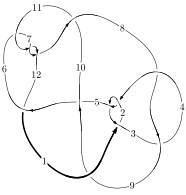
\includegraphics[width=112pt]{../../../GIT/diagram.site/Diagrams/png/946_12a_0145.png}\\
\ \ \ A knot diagram\footnotemark}&
\allowdisplaybreaks
\textbf{Linearized knot diagam} \\
\cline{2-2}
 &
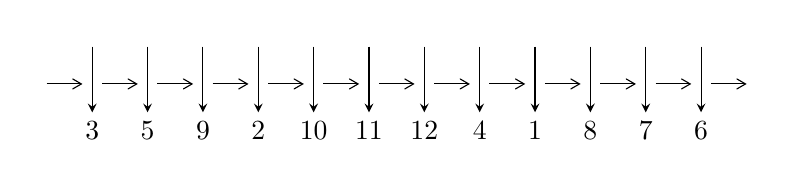
\begin{tikzpicture}[x=20pt, y=17pt]
	% nodes
	\node (C0) at (0, 0) {};
	\node (C1) at (1, 0) {};
	\node (C1U) at (1, +1) {};
	\node (C1D) at (1, -1) {3};

	\node (C2) at (2, 0) {};
	\node (C2U) at (2, +1) {};
	\node (C2D) at (2, -1) {5};

	\node (C3) at (3, 0) {};
	\node (C3U) at (3, +1) {};
	\node (C3D) at (3, -1) {9};

	\node (C4) at (4, 0) {};
	\node (C4U) at (4, +1) {};
	\node (C4D) at (4, -1) {2};

	\node (C5) at (5, 0) {};
	\node (C5U) at (5, +1) {};
	\node (C5D) at (5, -1) {10};

	\node (C6) at (6, 0) {};
	\node (C6U) at (6, +1) {};
	\node (C6D) at (6, -1) {11};

	\node (C7) at (7, 0) {};
	\node (C7U) at (7, +1) {};
	\node (C7D) at (7, -1) {12};

	\node (C8) at (8, 0) {};
	\node (C8U) at (8, +1) {};
	\node (C8D) at (8, -1) {4};

	\node (C9) at (9, 0) {};
	\node (C9U) at (9, +1) {};
	\node (C9D) at (9, -1) {1};

	\node (C10) at (10, 0) {};
	\node (C10U) at (10, +1) {};
	\node (C10D) at (10, -1) {8};

	\node (C11) at (11, 0) {};
	\node (C11U) at (11, +1) {};
	\node (C11D) at (11, -1) {7};

	\node (C12) at (12, 0) {};
	\node (C12U) at (12, +1) {};
	\node (C12D) at (12, -1) {6};
	\node (C13) at (13, 0) {};

	% arrows
	\draw[->,>={angle 60}]
	(C0) edge (C1) (C1) edge (C2) (C2) edge (C3) (C3) edge (C4) (C4) edge (C5) (C5) edge (C6) (C6) edge (C7) (C7) edge (C8) (C8) edge (C9) (C9) edge (C10) (C10) edge (C11) (C11) edge (C12) (C12) edge (C13) ;	\draw[->,>=stealth]
	(C1U) edge (C1D) (C2U) edge (C2D) (C3U) edge (C3D) (C4U) edge (C4D) (C5U) edge (C5D) (C6U) edge (C6D) (C7U) edge (C7D) (C8U) edge (C8D) (C9U) edge (C9D) (C10U) edge (C10D) (C11U) edge (C11D) (C12U) edge (C12D) ;
	\end{tikzpicture} \\
\hhline{~~} \\& 
\textbf{Solving Sequence} \\ \cline{2-2} 
 &
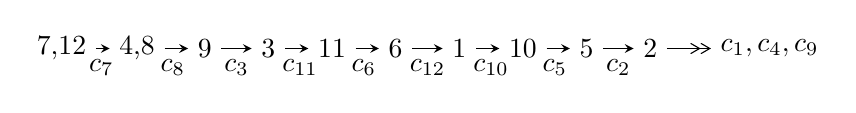
\begin{tikzpicture}[x=23pt, y=7pt]
	% node
	\node (A0) at (-1/8, 0) {7,12};
	\node (A1) at (17/16, 0) {4,8};
	\node (A2) at (17/8, 0) {9};
	\node (A3) at (25/8, 0) {3};
	\node (A4) at (33/8, 0) {11};
	\node (A5) at (41/8, 0) {6};
	\node (A6) at (49/8, 0) {1};
	\node (A7) at (57/8, 0) {10};
	\node (A8) at (65/8, 0) {5};
	\node (A9) at (73/8, 0) {2};
	\node (C1) at (1/2, -1) {$c_{7}$};
	\node (C2) at (13/8, -1) {$c_{8}$};
	\node (C3) at (21/8, -1) {$c_{3}$};
	\node (C4) at (29/8, -1) {$c_{11}$};
	\node (C5) at (37/8, -1) {$c_{6}$};
	\node (C6) at (45/8, -1) {$c_{12}$};
	\node (C7) at (53/8, -1) {$c_{10}$};
	\node (C8) at (61/8, -1) {$c_{5}$};
	\node (C9) at (69/8, -1) {$c_{2}$};
	\node (A10) at (11, 0) {$c_{1},c_{4},c_{9}$};

	% edge
	\draw[->,>=stealth]	
	(A0) edge (A1) (A1) edge (A2) (A2) edge (A3) (A3) edge (A4) (A4) edge (A5) (A5) edge (A6) (A6) edge (A7) (A7) edge (A8) (A8) edge (A9) ;
	\draw[->>,>={angle 60}]	
	(A9) edge (A10);
\end{tikzpicture} \\ 

\end{tabular} \\

\footnotetext{
The image of knot diagram is generated by the software ``\textbf{Draw programme}" developed by Andrew Bartholomew(\url{http://www.layer8.co.uk/maths/draw/index.htm\#Running-draw}), where we modified some parts for our purpose(\url{https://github.com/CATsTAILs/LinksPainter}).
}\phantom \\ \newline 
\centering \textbf{Ideals for irreducible components\footnotemark of $X_{\text{par}}$} 
 
\begin{align*}
I^u_{1}&=\langle 
- u^{95}+37 u^{93}+\cdots+b- u,\;- u^{95}+u^{94}+\cdots+a+1,\;u^{97}-2 u^{96}+\cdots+u-1\rangle \\
I^u_{2}&=\langle 
u^7-2 u^5+u^4+u^3- u^2+b+u,\;u^7+u^6-2 u^5-2 u^4+u^3+u^2+a+u+1,\\
\phantom{I^u_{2}}&\phantom{= \langle  }u^8+u^7-3 u^6-2 u^5+3 u^4+2 u-1\rangle \\
\\
\end{align*}
\raggedright * 2 irreducible components of $\dim_{\mathbb{C}}=0$, with total 105 representations.\\
\footnotetext{All coefficients of polynomials are rational numbers. But the coefficients are sometimes approximated in decimal forms when there is not enough margin.}
\newpage
\renewcommand{\arraystretch}{1}
\centering \section*{I. $I^u_{1}= \langle - u^{95}+37 u^{93}+\cdots+b- u,\;- u^{95}+u^{94}+\cdots+a+1,\;u^{97}-2 u^{96}+\cdots+u-1 \rangle$}
\flushleft \textbf{(i) Arc colorings}\\
\begin{tabular}{m{7pt} m{180pt} m{7pt} m{180pt} }
\flushright $a_{7}=$&$\begin{pmatrix}1\\0\end{pmatrix}$ \\
\flushright $a_{12}=$&$\begin{pmatrix}0\\u\end{pmatrix}$ \\
\flushright $a_{4}=$&$\begin{pmatrix}u^{95}- u^{94}+\cdots+u-1\\u^{95}-37 u^{93}+\cdots- u^2+u\end{pmatrix}$ \\
\flushright $a_{8}=$&$\begin{pmatrix}1\\u^2\end{pmatrix}$ \\
\flushright $a_{9}=$&$\begin{pmatrix}- u^{15}+6 u^{13}-14 u^{11}+14 u^9-2 u^7-6 u^5+2 u^3+2 u\\- u^{15}+5 u^{13}-8 u^{11}+u^9+8 u^7-4 u^5-2 u^3+u\end{pmatrix}$ \\
\flushright $a_{3}=$&$\begin{pmatrix}u^{95}- u^{94}+\cdots+5 u^3- u^2\\2 u^{96}- u^{95}+\cdots-8 u^2+2\end{pmatrix}$ \\
\flushright $a_{11}=$&$\begin{pmatrix}u\\u\end{pmatrix}$ \\
\flushright $a_{6}=$&$\begin{pmatrix}- u^2+1\\- u^2\end{pmatrix}$ \\
\flushright $a_{1}=$&$\begin{pmatrix}- u^5+2 u^3- u\\- u^5+u^3+u\end{pmatrix}$ \\
\flushright $a_{10}=$&$\begin{pmatrix}- u^3+2 u\\- u^5+u^3+u\end{pmatrix}$ \\
\flushright $a_{5}=$&$\begin{pmatrix}u^{10}-5 u^8+8 u^6-3 u^4-3 u^2+1\\u^{12}-4 u^{10}+4 u^8+2 u^6-3 u^4-2 u^2\end{pmatrix}$ \\
\flushright $a_{2}=$&$\begin{pmatrix}u^{95}- u^{94}+\cdots-4 u^2+u\\u^{96}-39 u^{94}+\cdots+u+1\end{pmatrix}$\\&\end{tabular}
\flushleft \textbf{(ii) Obstruction class $= -1$}\\~\\
\flushleft \textbf{(iii) Cusp Shapes $= 9 u^{96}-8 u^{95}+\cdots-13 u-7$}\\~\\
\newpage\renewcommand{\arraystretch}{1}
\flushleft \textbf{(iv) u-Polynomials at the component}\newline \\
\begin{tabular}{m{50pt}|m{274pt}}
Crossings & \hspace{64pt}u-Polynomials at each crossing \\
\hline $$\begin{aligned}c_{1}\end{aligned}$$&$\begin{aligned}
&u^{97}+45 u^{96}+\cdots+33 u+1
\end{aligned}$\\
\hline $$\begin{aligned}c_{2},c_{4}\end{aligned}$$&$\begin{aligned}
&u^{97}-9 u^{96}+\cdots- u+1
\end{aligned}$\\
\hline $$\begin{aligned}c_{3},c_{8}\end{aligned}$$&$\begin{aligned}
&u^{97}- u^{96}+\cdots+384 u+256
\end{aligned}$\\
\hline $$\begin{aligned}c_{5}\end{aligned}$$&$\begin{aligned}
&u^{97}-2 u^{96}+\cdots+1189 u+137
\end{aligned}$\\
\hline $$\begin{aligned}c_{6},c_{7},c_{11}\end{aligned}$$&$\begin{aligned}
&u^{97}+2 u^{96}+\cdots+u+1
\end{aligned}$\\
\hline $$\begin{aligned}c_{9}\end{aligned}$$&$\begin{aligned}
&u^{97}+8 u^{96}+\cdots+1059257 u+154033
\end{aligned}$\\
\hline $$\begin{aligned}c_{10},c_{12}\end{aligned}$$&$\begin{aligned}
&u^{97}-6 u^{96}+\cdots-239 u+77
\end{aligned}$\\
\hline
\end{tabular}\\~\\
\newpage\renewcommand{\arraystretch}{1}
\flushleft \textbf{(v) Riley Polynomials at the component}\newline \\
\begin{tabular}{m{50pt}|m{274pt}}
Crossings & \hspace{64pt}Riley Polynomials at each crossing \\
\hline $$\begin{aligned}c_{1}\end{aligned}$$&$\begin{aligned}
&y^{97}+23 y^{96}+\cdots+1253 y-1
\end{aligned}$\\
\hline $$\begin{aligned}c_{2},c_{4}\end{aligned}$$&$\begin{aligned}
&y^{97}-45 y^{96}+\cdots+33 y-1
\end{aligned}$\\
\hline $$\begin{aligned}c_{3},c_{8}\end{aligned}$$&$\begin{aligned}
&y^{97}+51 y^{96}+\cdots-1130496 y-65536
\end{aligned}$\\
\hline $$\begin{aligned}c_{5}\end{aligned}$$&$\begin{aligned}
&y^{97}+98 y^{95}+\cdots-285079 y-18769
\end{aligned}$\\
\hline $$\begin{aligned}c_{6},c_{7},c_{11}\end{aligned}$$&$\begin{aligned}
&y^{97}-80 y^{96}+\cdots+9 y-1
\end{aligned}$\\
\hline $$\begin{aligned}c_{9}\end{aligned}$$&$\begin{aligned}
&y^{97}+36 y^{96}+\cdots-192418294111 y-23726165089
\end{aligned}$\\
\hline $$\begin{aligned}c_{10},c_{12}\end{aligned}$$&$\begin{aligned}
&y^{97}+64 y^{96}+\cdots+69133 y-5929
\end{aligned}$\\
\hline
\end{tabular}\\~\\
\newpage\flushleft \textbf{(vi) Complex Volumes and Cusp Shapes}
$$\begin{array}{c|c|c}  
\text{Solutions to }I^u_{1}& \I (\text{vol} + \sqrt{-1}CS) & \text{Cusp shape}\\
 \hline 
\begin{aligned}
u &= \phantom{-}1.076300 + 0.183005 I \\
a &= \phantom{-}0.130363 - 0.085867 I \\
b &= -0.006250 - 0.958976 I\end{aligned}
 & -1.51529 - 2.04174 I & \phantom{-0.000000 } 0 \\ \hline\begin{aligned}
u &= \phantom{-}1.076300 - 0.183005 I \\
a &= \phantom{-}0.130363 + 0.085867 I \\
b &= -0.006250 + 0.958976 I\end{aligned}
 & -1.51529 + 2.04174 I & \phantom{-0.000000 } 0 \\ \hline\begin{aligned}
u &= -1.118950 + 0.358927 I \\
a &= \phantom{-}0.204765 - 1.283210 I \\
b &= -1.44474 - 2.86226 I\end{aligned}
 & \phantom{-}2.58320 - 8.29355 I & \phantom{-0.000000 } 0 \\ \hline\begin{aligned}
u &= -1.118950 - 0.358927 I \\
a &= \phantom{-}0.204765 + 1.283210 I \\
b &= -1.44474 + 2.86226 I\end{aligned}
 & \phantom{-}2.58320 + 8.29355 I & \phantom{-0.000000 } 0 \\ \hline\begin{aligned}
u &= -0.126507 + 0.813406 I \\
a &= -0.88778 - 2.82040 I \\
b &= \phantom{-}0.656917 + 0.751120 I\end{aligned}
 & \phantom{-}5.60707 + 12.55680 I & -7.94553 - 8.56908 I \\ \hline\begin{aligned}
u &= -0.126507 - 0.813406 I \\
a &= -0.88778 + 2.82040 I \\
b &= \phantom{-}0.656917 - 0.751120 I\end{aligned}
 & \phantom{-}5.60707 - 12.55680 I & -7.94553 + 8.56908 I \\ \hline\begin{aligned}
u &= -0.114542 + 0.813510 I \\
a &= \phantom{-}0.90688 + 2.89676 I \\
b &= -0.511057 - 0.767427 I\end{aligned}
 & \phantom{-}7.79765 + 6.77920 I & -4.92908 - 4.46483 I \\ \hline\begin{aligned}
u &= -0.114542 - 0.813510 I \\
a &= \phantom{-}0.90688 - 2.89676 I \\
b &= -0.511057 + 0.767427 I\end{aligned}
 & \phantom{-}7.79765 - 6.77920 I & -4.92908 + 4.46483 I \\ \hline\begin{aligned}
u &= -0.073078 + 0.816109 I \\
a &= \phantom{-}0.85010 + 2.82869 I \\
b &= -0.042433 - 0.632490 I\end{aligned}
 & \phantom{-}9.09233 + 2.43008 I & -3.53506 - 2.81478 I \\ \hline\begin{aligned}
u &= -0.073078 - 0.816109 I \\
a &= \phantom{-}0.85010 - 2.82869 I \\
b &= -0.042433 + 0.632490 I\end{aligned}
 & \phantom{-}9.09233 - 2.43008 I & -3.53506 + 2.81478 I\\
 \hline 
 \end{array}$$\newpage$$\begin{array}{c|c|c}  
\text{Solutions to }I^u_{1}& \I (\text{vol} + \sqrt{-1}CS) & \text{Cusp shape}\\
 \hline 
\begin{aligned}
u &= -0.053392 + 0.816761 I \\
a &= -0.86603 - 2.65617 I \\
b &= -0.104329 + 0.536098 I\end{aligned}
 & \phantom{-}7.87684 - 3.37088 I & -5.11230 + 2.63195 I \\ \hline\begin{aligned}
u &= -0.053392 - 0.816761 I \\
a &= -0.86603 + 2.65617 I \\
b &= -0.104329 - 0.536098 I\end{aligned}
 & \phantom{-}7.87684 + 3.37088 I & -5.11230 - 2.63195 I \\ \hline\begin{aligned}
u &= \phantom{-}0.111101 + 0.799935 I \\
a &= \phantom{-}1.288940 + 0.391351 I \\
b &= \phantom{-}0.188694 - 0.395318 I\end{aligned}
 & \phantom{-}2.82430 - 6.28995 I & -8.96385 + 6.07637 I \\ \hline\begin{aligned}
u &= \phantom{-}0.111101 - 0.799935 I \\
a &= \phantom{-}1.288940 - 0.391351 I \\
b &= \phantom{-}0.188694 + 0.395318 I\end{aligned}
 & \phantom{-}2.82430 + 6.28995 I & -8.96385 - 6.07637 I \\ \hline\begin{aligned}
u &= -1.137870 + 0.358762 I \\
a &= -0.05121 + 1.51386 I \\
b &= \phantom{-}1.60910 + 3.09123 I\end{aligned}
 & \phantom{-}4.67850 - 2.52431 I & \phantom{-0.000000 } 0 \\ \hline\begin{aligned}
u &= -1.137870 - 0.358762 I \\
a &= -0.05121 - 1.51386 I \\
b &= \phantom{-}1.60910 - 3.09123 I\end{aligned}
 & \phantom{-}4.67850 + 2.52431 I & \phantom{-0.000000 } 0 \\ \hline\begin{aligned}
u &= \phantom{-}1.144730 + 0.337722 I \\
a &= -0.109726 - 0.311521 I \\
b &= -0.944110 - 0.801712 I\end{aligned}
 & -0.31619 + 2.14672 I & \phantom{-0.000000 } 0 \\ \hline\begin{aligned}
u &= \phantom{-}1.144730 - 0.337722 I \\
a &= -0.109726 + 0.311521 I \\
b &= -0.944110 + 0.801712 I\end{aligned}
 & -0.31619 - 2.14672 I & \phantom{-0.000000 } 0 \\ \hline\begin{aligned}
u &= -0.103420 + 0.790241 I \\
a &= -0.96997 - 3.10450 I \\
b &= \phantom{-}0.323567 + 1.128250 I\end{aligned}
 & \phantom{-}1.70977 + 3.78539 I & -7.61756 - 4.82864 I \\ \hline\begin{aligned}
u &= -0.103420 - 0.790241 I \\
a &= -0.96997 + 3.10450 I \\
b &= \phantom{-}0.323567 - 1.128250 I\end{aligned}
 & \phantom{-}1.70977 - 3.78539 I & -7.61756 + 4.82864 I\\
 \hline 
 \end{array}$$\newpage$$\begin{array}{c|c|c}  
\text{Solutions to }I^u_{1}& \I (\text{vol} + \sqrt{-1}CS) & \text{Cusp shape}\\
 \hline 
\begin{aligned}
u &= \phantom{-}0.085353 + 0.791661 I \\
a &= -1.038950 - 0.762296 I \\
b &= -0.252154 + 0.312520 I\end{aligned}
 & \phantom{-}3.68280 - 1.75925 I & -7.15174 + 0.63615 I \\ \hline\begin{aligned}
u &= \phantom{-}0.085353 - 0.791661 I \\
a &= -1.038950 + 0.762296 I \\
b &= -0.252154 - 0.312520 I\end{aligned}
 & \phantom{-}3.68280 + 1.75925 I & -7.15174 - 0.63615 I \\ \hline\begin{aligned}
u &= -1.160010 + 0.325334 I \\
a &= \phantom{-}0.19316 - 2.24370 I \\
b &= -1.63673 - 3.84153 I\end{aligned}
 & -1.49498 + 0.27763 I & \phantom{-0.000000 } 0 \\ \hline\begin{aligned}
u &= -1.160010 - 0.325334 I \\
a &= \phantom{-}0.19316 + 2.24370 I \\
b &= -1.63673 + 3.84153 I\end{aligned}
 & -1.49498 - 0.27763 I & \phantom{-0.000000 } 0 \\ \hline\begin{aligned}
u &= \phantom{-}1.182250 + 0.335072 I \\
a &= \phantom{-}0.255858 + 0.190904 I \\
b &= \phantom{-}1.180070 + 0.374378 I\end{aligned}
 & \phantom{-}0.33868 - 2.32547 I & \phantom{-0.000000 } 0 \\ \hline\begin{aligned}
u &= \phantom{-}1.182250 - 0.335072 I \\
a &= \phantom{-}0.255858 - 0.190904 I \\
b &= \phantom{-}1.180070 - 0.374378 I\end{aligned}
 & \phantom{-}0.33868 + 2.32547 I & \phantom{-0.000000 } 0 \\ \hline\begin{aligned}
u &= \phantom{-}0.143920 + 0.749716 I \\
a &= \phantom{-}0.840542 - 0.473330 I \\
b &= -0.143901 - 0.352024 I\end{aligned}
 & \phantom{-}1.23810 - 1.61799 I & -7.46158 - 0.93127 I \\ \hline\begin{aligned}
u &= \phantom{-}0.143920 - 0.749716 I \\
a &= \phantom{-}0.840542 + 0.473330 I \\
b &= -0.143901 + 0.352024 I\end{aligned}
 & \phantom{-}1.23810 + 1.61799 I & -7.46158 + 0.93127 I \\ \hline\begin{aligned}
u &= -1.190710 + 0.363826 I \\
a &= \phantom{-}0.53577 + 1.88222 I \\
b &= \phantom{-}2.10121 + 3.28700 I\end{aligned}
 & \phantom{-}5.66672 + 1.82828 I & \phantom{-0.000000 } 0 \\ \hline\begin{aligned}
u &= -1.190710 - 0.363826 I \\
a &= \phantom{-}0.53577 - 1.88222 I \\
b &= \phantom{-}2.10121 - 3.28700 I\end{aligned}
 & \phantom{-}5.66672 - 1.82828 I & \phantom{-0.000000 } 0\\
 \hline 
 \end{array}$$\newpage$$\begin{array}{c|c|c}  
\text{Solutions to }I^u_{1}& \I (\text{vol} + \sqrt{-1}CS) & \text{Cusp shape}\\
 \hline 
\begin{aligned}
u &= \phantom{-}1.234940 + 0.251161 I \\
a &= \phantom{-}0.0367038 - 0.0468935 I \\
b &= \phantom{-}0.429880 - 0.656423 I\end{aligned}
 & -1.31278 - 1.68000 I & \phantom{-0.000000 } 0 \\ \hline\begin{aligned}
u &= \phantom{-}1.234940 - 0.251161 I \\
a &= \phantom{-}0.0367038 + 0.0468935 I \\
b &= \phantom{-}0.429880 + 0.656423 I\end{aligned}
 & -1.31278 + 1.68000 I & \phantom{-0.000000 } 0 \\ \hline\begin{aligned}
u &= -1.210910 + 0.365700 I \\
a &= -0.69971 - 1.90645 I \\
b &= -2.14117 - 3.22189 I\end{aligned}
 & \phantom{-}4.31801 + 7.63181 I & \phantom{-0.000000 } 0 \\ \hline\begin{aligned}
u &= -1.210910 - 0.365700 I \\
a &= -0.69971 + 1.90645 I \\
b &= -2.14117 + 3.22189 I\end{aligned}
 & \phantom{-}4.31801 - 7.63181 I & \phantom{-0.000000 } 0 \\ \hline\begin{aligned}
u &= \phantom{-}0.067904 + 0.716739 I \\
a &= \phantom{-}0.005795 - 1.052530 I \\
b &= -0.418357 + 0.045210 I\end{aligned}
 & \phantom{-}2.22161 - 1.81122 I & -6.58757 + 4.34433 I \\ \hline\begin{aligned}
u &= \phantom{-}0.067904 - 0.716739 I \\
a &= \phantom{-}0.005795 + 1.052530 I \\
b &= -0.418357 - 0.045210 I\end{aligned}
 & \phantom{-}2.22161 + 1.81122 I & -6.58757 - 4.34433 I \\ \hline\begin{aligned}
u &= \phantom{-}0.694155 + 0.155276 I \\
a &= -0.129694 - 0.373429 I \\
b &= -0.284181 + 0.715904 I\end{aligned}
 & -1.64822 + 1.85592 I & -13.39585 - 2.90468 I \\ \hline\begin{aligned}
u &= \phantom{-}0.694155 - 0.155276 I \\
a &= -0.129694 + 0.373429 I \\
b &= -0.284181 - 0.715904 I\end{aligned}
 & -1.64822 - 1.85592 I & -13.39585 + 2.90468 I \\ \hline\begin{aligned}
u &= \phantom{-}0.166510 + 0.680908 I \\
a &= -0.652095 + 1.069380 I \\
b &= \phantom{-}0.462505 + 0.336470 I\end{aligned}
 & \phantom{-}0.37978 - 5.08479 I & -10.13756 + 7.85339 I \\ \hline\begin{aligned}
u &= \phantom{-}0.166510 - 0.680908 I \\
a &= -0.652095 - 1.069380 I \\
b &= \phantom{-}0.462505 - 0.336470 I\end{aligned}
 & \phantom{-}0.37978 + 5.08479 I & -10.13756 - 7.85339 I\\
 \hline 
 \end{array}$$\newpage$$\begin{array}{c|c|c}  
\text{Solutions to }I^u_{1}& \I (\text{vol} + \sqrt{-1}CS) & \text{Cusp shape}\\
 \hline 
\begin{aligned}
u &= \phantom{-}1.290550 + 0.155428 I \\
a &= \phantom{-}0.330614 + 0.169609 I \\
b &= \phantom{-}0.634930 - 0.619092 I\end{aligned}
 & -1.26131 - 1.89849 I & \phantom{-0.000000 } 0 \\ \hline\begin{aligned}
u &= \phantom{-}1.290550 - 0.155428 I \\
a &= \phantom{-}0.330614 - 0.169609 I \\
b &= \phantom{-}0.634930 + 0.619092 I\end{aligned}
 & -1.26131 + 1.89849 I & \phantom{-0.000000 } 0 \\ \hline\begin{aligned}
u &= -1.299620 + 0.260517 I \\
a &= \phantom{-}1.71939 + 0.85305 I \\
b &= \phantom{-}2.59874 + 0.76974 I\end{aligned}
 & -4.80583 + 2.13843 I & \phantom{-0.000000 } 0 \\ \hline\begin{aligned}
u &= -1.299620 - 0.260517 I \\
a &= \phantom{-}1.71939 - 0.85305 I \\
b &= \phantom{-}2.59874 - 0.76974 I\end{aligned}
 & -4.80583 - 2.13843 I & \phantom{-0.000000 } 0 \\ \hline\begin{aligned}
u &= -1.335730 + 0.026914 I \\
a &= \phantom{-}1.229910 + 0.335097 I \\
b &= \phantom{-}1.44608 + 0.35864 I\end{aligned}
 & -5.57709 + 0.21725 I & \phantom{-0.000000 } 0 \\ \hline\begin{aligned}
u &= -1.335730 - 0.026914 I \\
a &= \phantom{-}1.229910 - 0.335097 I \\
b &= \phantom{-}1.44608 - 0.35864 I\end{aligned}
 & -5.57709 - 0.21725 I & \phantom{-0.000000 } 0 \\ \hline\begin{aligned}
u &= \phantom{-}1.310410 + 0.279225 I \\
a &= \phantom{-}0.688209 + 0.224075 I \\
b &= \phantom{-}0.37451 + 1.55998 I\end{aligned}
 & -5.06350 - 4.46571 I & \phantom{-0.000000 } 0 \\ \hline\begin{aligned}
u &= \phantom{-}1.310410 - 0.279225 I \\
a &= \phantom{-}0.688209 - 0.224075 I \\
b &= \phantom{-}0.37451 - 1.55998 I\end{aligned}
 & -5.06350 + 4.46571 I & \phantom{-0.000000 } 0 \\ \hline\begin{aligned}
u &= -0.535358 + 0.374511 I \\
a &= \phantom{-}1.62509 + 1.47845 I \\
b &= \phantom{-}0.223110 + 0.775600 I\end{aligned}
 & \phantom{-}1.26298 + 8.74212 I & -11.9170 - 9.0216 I \\ \hline\begin{aligned}
u &= -0.535358 - 0.374511 I \\
a &= \phantom{-}1.62509 - 1.47845 I \\
b &= \phantom{-}0.223110 - 0.775600 I\end{aligned}
 & \phantom{-}1.26298 - 8.74212 I & -11.9170 + 9.0216 I\\
 \hline 
 \end{array}$$\newpage$$\begin{array}{c|c|c}  
\text{Solutions to }I^u_{1}& \I (\text{vol} + \sqrt{-1}CS) & \text{Cusp shape}\\
 \hline 
\begin{aligned}
u &= -1.312070 + 0.304653 I \\
a &= -0.978270 - 0.798937 I \\
b &= -1.60919 - 0.98606 I\end{aligned}
 & -2.10580 + 5.52005 I & \phantom{-0.000000 } 0 \\ \hline\begin{aligned}
u &= -1.312070 - 0.304653 I \\
a &= -0.978270 + 0.798937 I \\
b &= -1.60919 + 0.98606 I\end{aligned}
 & -2.10580 - 5.52005 I & \phantom{-0.000000 } 0 \\ \hline\begin{aligned}
u &= \phantom{-}1.301650 + 0.360247 I \\
a &= \phantom{-}1.24554 - 0.95339 I \\
b &= \phantom{-}3.26147 - 1.62863 I\end{aligned}
 & \phantom{-}3.64680 - 0.86350 I & \phantom{-0.000000 } 0 \\ \hline\begin{aligned}
u &= \phantom{-}1.301650 - 0.360247 I \\
a &= \phantom{-}1.24554 + 0.95339 I \\
b &= \phantom{-}3.26147 + 1.62863 I\end{aligned}
 & \phantom{-}3.64680 + 0.86350 I & \phantom{-0.000000 } 0 \\ \hline\begin{aligned}
u &= \phantom{-}1.333670 + 0.214386 I \\
a &= \phantom{-}0.091767 - 0.625950 I \\
b &= -0.0419970 + 0.0777167 I\end{aligned}
 & -2.98555 + 2.91120 I & \phantom{-0.000000 } 0 \\ \hline\begin{aligned}
u &= \phantom{-}1.333670 - 0.214386 I \\
a &= \phantom{-}0.091767 + 0.625950 I \\
b &= -0.0419970 - 0.0777167 I\end{aligned}
 & -2.98555 - 2.91120 I & \phantom{-0.000000 } 0 \\ \hline\begin{aligned}
u &= -0.040986 + 0.644398 I \\
a &= -0.470789 + 1.316680 I \\
b &= \phantom{-}0.877565 + 0.056288 I\end{aligned}
 & -0.789349 + 1.067810 I & -12.54494 - 0.17404 I \\ \hline\begin{aligned}
u &= -0.040986 - 0.644398 I \\
a &= -0.470789 - 1.316680 I \\
b &= \phantom{-}0.877565 - 0.056288 I\end{aligned}
 & -0.789349 - 1.067810 I & -12.54494 + 0.17404 I \\ \hline\begin{aligned}
u &= \phantom{-}1.361170 + 0.045050 I \\
a &= -1.68001 + 0.84178 I \\
b &= -2.82631 + 2.17159 I\end{aligned}
 & -7.87318 - 1.71980 I & \phantom{-0.000000 } 0 \\ \hline\begin{aligned}
u &= \phantom{-}1.361170 - 0.045050 I \\
a &= -1.68001 - 0.84178 I \\
b &= -2.82631 - 2.17159 I\end{aligned}
 & -7.87318 + 1.71980 I & \phantom{-0.000000 } 0\\
 \hline 
 \end{array}$$\newpage$$\begin{array}{c|c|c}  
\text{Solutions to }I^u_{1}& \I (\text{vol} + \sqrt{-1}CS) & \text{Cusp shape}\\
 \hline 
\begin{aligned}
u &= \phantom{-}1.315640 + 0.358977 I \\
a &= -1.47555 + 1.24858 I \\
b &= -3.69497 + 1.94814 I\end{aligned}
 & \phantom{-}4.74652 - 6.65977 I & \phantom{-0.000000 } 0 \\ \hline\begin{aligned}
u &= \phantom{-}1.315640 - 0.358977 I \\
a &= -1.47555 - 1.24858 I \\
b &= -3.69497 - 1.94814 I\end{aligned}
 & \phantom{-}4.74652 + 6.65977 I & \phantom{-0.000000 } 0 \\ \hline\begin{aligned}
u &= -1.323330 + 0.342677 I \\
a &= -0.124269 - 1.289700 I \\
b &= -0.37275 - 1.97282 I\end{aligned}
 & -0.73515 + 5.85059 I & \phantom{-0.000000 } 0 \\ \hline\begin{aligned}
u &= -1.323330 - 0.342677 I \\
a &= -0.124269 + 1.289700 I \\
b &= -0.37275 + 1.97282 I\end{aligned}
 & -0.73515 - 5.85059 I & \phantom{-0.000000 } 0 \\ \hline\begin{aligned}
u &= -1.368030 + 0.059939 I \\
a &= -1.29273 - 0.90938 I \\
b &= -1.60119 - 1.03501 I\end{aligned}
 & -7.09539 + 4.13757 I & \phantom{-0.000000 } 0 \\ \hline\begin{aligned}
u &= -1.368030 - 0.059939 I \\
a &= -1.29273 + 0.90938 I \\
b &= -1.60119 + 1.03501 I\end{aligned}
 & -7.09539 - 4.13757 I & \phantom{-0.000000 } 0 \\ \hline\begin{aligned}
u &= \phantom{-}1.374290 + 0.079537 I \\
a &= \phantom{-}1.62166 + 0.00987 I \\
b &= \phantom{-}2.59757 - 0.79140 I\end{aligned}
 & -2.53211 - 4.62583 I & \phantom{-0.000000 } 0 \\ \hline\begin{aligned}
u &= \phantom{-}1.374290 - 0.079537 I \\
a &= \phantom{-}1.62166 - 0.00987 I \\
b &= \phantom{-}2.59757 + 0.79140 I\end{aligned}
 & -2.53211 + 4.62583 I & \phantom{-0.000000 } 0 \\ \hline\begin{aligned}
u &= \phantom{-}1.333520 + 0.341806 I \\
a &= \phantom{-}1.77954 - 2.08217 I \\
b &= \phantom{-}4.58642 - 2.78774 I\end{aligned}
 & -2.80433 - 7.87203 I & \phantom{-0.000000 } 0 \\ \hline\begin{aligned}
u &= \phantom{-}1.333520 - 0.341806 I \\
a &= \phantom{-}1.77954 + 2.08217 I \\
b &= \phantom{-}4.58642 + 2.78774 I\end{aligned}
 & -2.80433 + 7.87203 I & \phantom{-0.000000 } 0\\
 \hline 
 \end{array}$$\newpage$$\begin{array}{c|c|c}  
\text{Solutions to }I^u_{1}& \I (\text{vol} + \sqrt{-1}CS) & \text{Cusp shape}\\
 \hline 
\begin{aligned}
u &= -1.348380 + 0.289480 I \\
a &= \phantom{-}1.44252 + 0.02874 I \\
b &= \phantom{-}2.06872 - 0.16790 I\end{aligned}
 & -4.37828 + 8.63452 I & \phantom{-0.000000 } 0 \\ \hline\begin{aligned}
u &= -1.348380 - 0.289480 I \\
a &= \phantom{-}1.44252 - 0.02874 I \\
b &= \phantom{-}2.06872 + 0.16790 I\end{aligned}
 & -4.37828 - 8.63452 I & \phantom{-0.000000 } 0 \\ \hline\begin{aligned}
u &= -1.338200 + 0.346591 I \\
a &= -0.258393 + 1.359040 I \\
b &= -0.24512 + 2.10842 I\end{aligned}
 & -1.73047 + 10.42640 I & \phantom{-0.000000 } 0 \\ \hline\begin{aligned}
u &= -1.338200 - 0.346591 I \\
a &= -0.258393 - 1.359040 I \\
b &= -0.24512 - 2.10842 I\end{aligned}
 & -1.73047 - 10.42640 I & \phantom{-0.000000 } 0 \\ \hline\begin{aligned}
u &= -0.484186 + 0.378282 I \\
a &= -1.50954 - 1.53900 I \\
b &= -0.322758 - 0.792431 I\end{aligned}
 & \phantom{-}3.24484 + 3.24235 I & -8.65530 - 4.94862 I \\ \hline\begin{aligned}
u &= -0.484186 - 0.378282 I \\
a &= -1.50954 + 1.53900 I \\
b &= -0.322758 + 0.792431 I\end{aligned}
 & \phantom{-}3.24484 - 3.24235 I & -8.65530 + 4.94862 I \\ \hline\begin{aligned}
u &= -1.349460 + 0.319480 I \\
a &= -0.829122 + 0.586131 I \\
b &= -1.15265 + 0.96709 I\end{aligned}
 & -3.46530 + 5.49686 I & \phantom{-0.000000 } 0 \\ \hline\begin{aligned}
u &= -1.349460 - 0.319480 I \\
a &= -0.829122 - 0.586131 I \\
b &= -1.15265 - 0.96709 I\end{aligned}
 & -3.46530 - 5.49686 I & \phantom{-0.000000 } 0 \\ \hline\begin{aligned}
u &= \phantom{-}1.341310 + 0.353804 I \\
a &= -2.06581 + 1.68918 I \\
b &= -4.57878 + 2.14247 I\end{aligned}
 & \phantom{-}3.22187 - 10.98640 I & \phantom{-0.000000 } 0 \\ \hline\begin{aligned}
u &= \phantom{-}1.341310 - 0.353804 I \\
a &= -2.06581 - 1.68918 I \\
b &= -4.57878 - 2.14247 I\end{aligned}
 & \phantom{-}3.22187 + 10.98640 I & \phantom{-0.000000 } 0\\
 \hline 
 \end{array}$$\newpage$$\begin{array}{c|c|c}  
\text{Solutions to }I^u_{1}& \I (\text{vol} + \sqrt{-1}CS) & \text{Cusp shape}\\
 \hline 
\begin{aligned}
u &= \phantom{-}1.390800 + 0.073948 I \\
a &= -1.94759 - 0.11301 I \\
b &= -3.08499 + 0.56757 I\end{aligned}
 & -4.75509 - 10.05740 I & \phantom{-0.000000 } 0 \\ \hline\begin{aligned}
u &= \phantom{-}1.390800 - 0.073948 I \\
a &= -1.94759 + 0.11301 I \\
b &= -3.08499 - 0.56757 I\end{aligned}
 & -4.75509 + 10.05740 I & \phantom{-0.000000 } 0 \\ \hline\begin{aligned}
u &= \phantom{-}1.348030 + 0.352429 I \\
a &= \phantom{-}2.21445 - 1.72567 I \\
b &= \phantom{-}4.71204 - 2.06495 I\end{aligned}
 & \phantom{-}0.9676 - 16.7600 I & \phantom{-0.000000 } 0 \\ \hline\begin{aligned}
u &= \phantom{-}1.348030 - 0.352429 I \\
a &= \phantom{-}2.21445 + 1.72567 I \\
b &= \phantom{-}4.71204 + 2.06495 I\end{aligned}
 & \phantom{-}0.9676 + 16.7600 I & \phantom{-0.000000 } 0 \\ \hline\begin{aligned}
u &= -1.395620 + 0.017256 I \\
a &= -0.419590 - 1.142350 I \\
b &= -0.52309 - 1.38433 I\end{aligned}
 & -7.89376 - 1.50579 I & \phantom{-0.000000 } 0 \\ \hline\begin{aligned}
u &= -1.395620 - 0.017256 I \\
a &= -0.419590 + 1.142350 I \\
b &= -0.52309 + 1.38433 I\end{aligned}
 & -7.89376 + 1.50579 I & \phantom{-0.000000 } 0 \\ \hline\begin{aligned}
u &= -0.303128 + 0.514916 I \\
a &= \phantom{-}0.760246 + 1.014040 I \\
b &= \phantom{-}0.734346 + 0.775395 I\end{aligned}
 & \phantom{-}1.99642 - 5.50453 I & -9.70697 + 2.05579 I \\ \hline\begin{aligned}
u &= -0.303128 - 0.514916 I \\
a &= \phantom{-}0.760246 - 1.014040 I \\
b &= \phantom{-}0.734346 - 0.775395 I\end{aligned}
 & \phantom{-}1.99642 + 5.50453 I & -9.70697 - 2.05579 I \\ \hline\begin{aligned}
u &= -0.338950 + 0.455365 I \\
a &= -0.93268 - 1.30856 I \\
b &= -0.595427 - 0.780173 I\end{aligned}
 & \phantom{-}3.69304 - 0.15503 I & -6.96002 - 3.29097 I \\ \hline\begin{aligned}
u &= -0.338950 - 0.455365 I \\
a &= -0.93268 + 1.30856 I \\
b &= -0.595427 + 0.780173 I\end{aligned}
 & \phantom{-}3.69304 + 0.15503 I & -6.96002 + 3.29097 I\\
 \hline 
 \end{array}$$\newpage$$\begin{array}{c|c|c}  
\text{Solutions to }I^u_{1}& \I (\text{vol} + \sqrt{-1}CS) & \text{Cusp shape}\\
 \hline 
\begin{aligned}
u &= \phantom{-}0.467931 + 0.308565 I \\
a &= \phantom{-}0.084687 - 0.878435 I \\
b &= -0.670638 + 0.271758 I\end{aligned}
 & -1.42451 - 3.05583 I & -14.0334 + 7.0667 I \\ \hline\begin{aligned}
u &= \phantom{-}0.467931 - 0.308565 I \\
a &= \phantom{-}0.084687 + 0.878435 I \\
b &= -0.670638 - 0.271758 I\end{aligned}
 & -1.42451 + 3.05583 I & -14.0334 - 7.0667 I \\ \hline\begin{aligned}
u &= -0.430554 + 0.233040 I \\
a &= \phantom{-}1.65460 + 2.24861 I \\
b &= \phantom{-}0.407916 + 0.668554 I\end{aligned}
 & -2.34524 + 0.90469 I & -12.7209 - 7.5741 I \\ \hline\begin{aligned}
u &= -0.430554 - 0.233040 I \\
a &= \phantom{-}1.65460 - 2.24861 I \\
b &= \phantom{-}0.407916 - 0.668554 I\end{aligned}
 & -2.34524 - 0.90469 I & -12.7209 + 7.5741 I \\ \hline\begin{aligned}
u &= \phantom{-}0.248050 + 0.339715 I \\
a &= -0.509169 + 1.177470 I \\
b &= \phantom{-}0.609743 + 0.066227 I\end{aligned}
 & -0.830925 + 0.497747 I & -11.61503 + 1.83140 I \\ \hline\begin{aligned}
u &= \phantom{-}0.248050 - 0.339715 I \\
a &= -0.509169 - 1.177470 I \\
b &= \phantom{-}0.609743 - 0.066227 I\end{aligned}
 & -0.830925 - 0.497747 I & -11.61503 - 1.83140 I \\ \hline\begin{aligned}
u &= \phantom{-}0.337597\phantom{ +0.000000I} \\
a &= -0.676853\phantom{ +0.000000I} \\
b &= \phantom{-}0.328344\phantom{ +0.000000I}\end{aligned}
 & -0.597166\phantom{ +0.000000I} & -16.5590\phantom{ +0.000000I}\\
 \hline 
 \end{array}$$\newpage\newpage\renewcommand{\arraystretch}{1}
\centering \section*{II. $I^u_{2}= \langle u^7-2 u^5+u^4+u^3- u^2+b+u,\;u^7+u^6-2 u^5-2 u^4+u^3+u^2+a+u+1,\;u^8+u^7-3 u^6-2 u^5+3 u^4+2 u-1 \rangle$}
\flushleft \textbf{(i) Arc colorings}\\
\begin{tabular}{m{7pt} m{180pt} m{7pt} m{180pt} }
\flushright $a_{7}=$&$\begin{pmatrix}1\\0\end{pmatrix}$ \\
\flushright $a_{12}=$&$\begin{pmatrix}0\\u\end{pmatrix}$ \\
\flushright $a_{4}=$&$\begin{pmatrix}- u^7- u^6+2 u^5+2 u^4- u^3- u^2- u-1\\- u^7+2 u^5- u^4- u^3+u^2- u\end{pmatrix}$ \\
\flushright $a_{8}=$&$\begin{pmatrix}1\\u^2\end{pmatrix}$ \\
\flushright $a_{9}=$&$\begin{pmatrix}1\\u^2\end{pmatrix}$ \\
\flushright $a_{3}=$&$\begin{pmatrix}- u^7- u^6+2 u^5+2 u^4- u^3- u^2- u-1\\- u^7+2 u^5- u^4- u^3+u^2- u\end{pmatrix}$ \\
\flushright $a_{11}=$&$\begin{pmatrix}u\\u\end{pmatrix}$ \\
\flushright $a_{6}=$&$\begin{pmatrix}- u^2+1\\- u^2\end{pmatrix}$ \\
\flushright $a_{1}=$&$\begin{pmatrix}- u^5+2 u^3- u\\- u^5+u^3+u\end{pmatrix}$ \\
\flushright $a_{10}=$&$\begin{pmatrix}- u^3+2 u\\- u^5+u^3+u\end{pmatrix}$ \\
\flushright $a_{5}=$&$\begin{pmatrix}u^5-2 u^3+u\\u^5- u^3- u\end{pmatrix}$ \\
\flushright $a_{2}=$&$\begin{pmatrix}- u^7- u^6+u^5+2 u^4+u^3- u^2-2 u-1\\- u^7+u^5- u^4+u^2\end{pmatrix}$\\&\end{tabular}
\flushleft \textbf{(ii) Obstruction class $= 1$}\\~\\
\flushleft \textbf{(iii) Cusp Shapes $= u^7-2 u^6-2 u^5+8 u^4-3 u^3-7 u^2+8 u-19$}\\~\\
\newpage\renewcommand{\arraystretch}{1}
\flushleft \textbf{(iv) u-Polynomials at the component}\newline \\
\begin{tabular}{m{50pt}|m{274pt}}
Crossings & \hspace{64pt}u-Polynomials at each crossing \\
\hline $$\begin{aligned}c_{1},c_{2}\end{aligned}$$&$\begin{aligned}
&(u-1)^8
\end{aligned}$\\
\hline $$\begin{aligned}c_{3},c_{8}\end{aligned}$$&$\begin{aligned}
&u^8
\end{aligned}$\\
\hline $$\begin{aligned}c_{4}\end{aligned}$$&$\begin{aligned}
&(u+1)^8
\end{aligned}$\\
\hline $$\begin{aligned}c_{5},c_{9}\end{aligned}$$&$\begin{aligned}
&u^8- u^7- u^6+2 u^5+u^4-2 u^3+2 u-1
\end{aligned}$\\
\hline $$\begin{aligned}c_{6},c_{7}\end{aligned}$$&$\begin{aligned}
&u^8+u^7-3 u^6-2 u^5+3 u^4+2 u-1
\end{aligned}$\\
\hline $$\begin{aligned}c_{10},c_{12}\end{aligned}$$&$\begin{aligned}
&u^8+3 u^7+7 u^6+10 u^5+11 u^4+10 u^3+6 u^2+4 u+1
\end{aligned}$\\
\hline $$\begin{aligned}c_{11}\end{aligned}$$&$\begin{aligned}
&u^8- u^7-3 u^6+2 u^5+3 u^4-2 u-1
\end{aligned}$\\
\hline
\end{tabular}\\~\\
\newpage\renewcommand{\arraystretch}{1}
\flushleft \textbf{(v) Riley Polynomials at the component}\newline \\
\begin{tabular}{m{50pt}|m{274pt}}
Crossings & \hspace{64pt}Riley Polynomials at each crossing \\
\hline $$\begin{aligned}c_{1},c_{2},c_{4}\end{aligned}$$&$\begin{aligned}
&(y-1)^8
\end{aligned}$\\
\hline $$\begin{aligned}c_{3},c_{8}\end{aligned}$$&$\begin{aligned}
&y^8
\end{aligned}$\\
\hline $$\begin{aligned}c_{5},c_{9}\end{aligned}$$&$\begin{aligned}
&y^8-3 y^7+7 y^6-10 y^5+11 y^4-10 y^3+6 y^2-4 y+1
\end{aligned}$\\
\hline $$\begin{aligned}c_{6},c_{7},c_{11}\end{aligned}$$&$\begin{aligned}
&y^8-7 y^7+19 y^6-22 y^5+3 y^4+14 y^3-6 y^2-4 y+1
\end{aligned}$\\
\hline $$\begin{aligned}c_{10},c_{12}\end{aligned}$$&$\begin{aligned}
&y^8+5 y^7+11 y^6+6 y^5-17 y^4-34 y^3-22 y^2-4 y+1
\end{aligned}$\\
\hline
\end{tabular}\\~\\
\newpage\flushleft \textbf{(vi) Complex Volumes and Cusp Shapes}
$$\begin{array}{c|c|c}  
\text{Solutions to }I^u_{2}& \I (\text{vol} + \sqrt{-1}CS) & \text{Cusp shape}\\
 \hline 
\begin{aligned}
u &= \phantom{-}1.180120 + 0.268597 I \\
a &= -0.663977 - 0.849844 I \\
b &= -0.33804 - 1.54318 I\end{aligned}
 & -2.68559 - 1.13123 I & -15.9046 + 0.8051 I \\ \hline\begin{aligned}
u &= \phantom{-}1.180120 - 0.268597 I \\
a &= -0.663977 + 0.849844 I \\
b &= -0.33804 + 1.54318 I\end{aligned}
 & -2.68559 + 1.13123 I & -15.9046 - 0.8051 I \\ \hline\begin{aligned}
u &= \phantom{-}0.108090 + 0.747508 I \\
a &= \phantom{-}0.727959 - 0.566792 I \\
b &= -0.306664 + 0.427719 I\end{aligned}
 & \phantom{-}0.51448 - 2.57849 I & -11.78039 + 3.88175 I \\ \hline\begin{aligned}
u &= \phantom{-}0.108090 - 0.747508 I \\
a &= \phantom{-}0.727959 + 0.566792 I \\
b &= -0.306664 - 0.427719 I\end{aligned}
 & \phantom{-}0.51448 + 2.57849 I & -11.78039 - 3.88175 I \\ \hline\begin{aligned}
u &= -1.37100\phantom{ +0.000000I} \\
a &= \phantom{-}0.910598\phantom{ +0.000000I} \\
b &= \phantom{-}1.71160\phantom{ +0.000000I}\end{aligned}
 & -8.14766\phantom{ +0.000000I} & -19.8290\phantom{ +0.000000I} \\ \hline\begin{aligned}
u &= -1.334530 + 0.318930 I \\
a &= -0.690511 - 0.438656 I \\
b &= -1.53294 - 0.14882 I\end{aligned}
 & -4.02461 + 6.44354 I & -16.5091 - 6.0410 I \\ \hline\begin{aligned}
u &= -1.334530 - 0.318930 I \\
a &= -0.690511 + 0.438656 I \\
b &= -1.53294 + 0.14882 I\end{aligned}
 & -4.02461 - 6.44354 I & -16.5091 + 6.0410 I \\ \hline\begin{aligned}
u &= \phantom{-}0.463640\phantom{ +0.000000I} \\
a &= -1.65754\phantom{ +0.000000I} \\
b &= -0.356309\phantom{ +0.000000I}\end{aligned}
 & -2.48997\phantom{ +0.000000I} & -16.7830\phantom{ +0.000000I}\\
 \hline 
 \end{array}$$\newpage
\newpage\renewcommand{\arraystretch}{1}
\centering \section*{ III. u-Polynomials}
\begin{tabular}{m{50pt}|m{274pt}}
Crossings & \hspace{64pt}u-Polynomials at each crossing \\
\hline $$\begin{aligned}c_{1}\end{aligned}$$&$\begin{aligned}
&((u-1)^8)(u^{97}+45 u^{96}+\cdots+33 u+1)
\end{aligned}$\\
\hline $$\begin{aligned}c_{2}\end{aligned}$$&$\begin{aligned}
&((u-1)^8)(u^{97}-9 u^{96}+\cdots- u+1)
\end{aligned}$\\
\hline $$\begin{aligned}c_{3},c_{8}\end{aligned}$$&$\begin{aligned}
&u^8(u^{97}- u^{96}+\cdots+384 u+256)
\end{aligned}$\\
\hline $$\begin{aligned}c_{4}\end{aligned}$$&$\begin{aligned}
&((u+1)^8)(u^{97}-9 u^{96}+\cdots- u+1)
\end{aligned}$\\
\hline $$\begin{aligned}c_{5}\end{aligned}$$&$\begin{aligned}
&(u^8- u^7- u^6+2 u^5+u^4-2 u^3+2 u-1)\\
&\cdot(u^{97}-2 u^{96}+\cdots+1189 u+137)
\end{aligned}$\\
\hline $$\begin{aligned}c_{6},c_{7}\end{aligned}$$&$\begin{aligned}
&(u^8+u^7-3 u^6-2 u^5+3 u^4+2 u-1)(u^{97}+2 u^{96}+\cdots+u+1)
\end{aligned}$\\
\hline $$\begin{aligned}c_{9}\end{aligned}$$&$\begin{aligned}
&(u^8- u^7- u^6+2 u^5+u^4-2 u^3+2 u-1)\\
&\cdot(u^{97}+8 u^{96}+\cdots+1059257 u+154033)
\end{aligned}$\\
\hline $$\begin{aligned}c_{10},c_{12}\end{aligned}$$&$\begin{aligned}
&(u^8+3 u^7+7 u^6+10 u^5+11 u^4+10 u^3+6 u^2+4 u+1)\\
&\cdot(u^{97}-6 u^{96}+\cdots-239 u+77)
\end{aligned}$\\
\hline $$\begin{aligned}c_{11}\end{aligned}$$&$\begin{aligned}
&(u^8- u^7-3 u^6+2 u^5+3 u^4-2 u-1)(u^{97}+2 u^{96}+\cdots+u+1)
\end{aligned}$\\
\hline
\end{tabular}\newpage\renewcommand{\arraystretch}{1}
\centering \section*{ IV. Riley Polynomials}
\begin{tabular}{m{50pt}|m{274pt}}
Crossings & \hspace{64pt}Riley Polynomials at each crossing \\
\hline $$\begin{aligned}c_{1}\end{aligned}$$&$\begin{aligned}
&((y-1)^8)(y^{97}+23 y^{96}+\cdots+1253 y-1)
\end{aligned}$\\
\hline $$\begin{aligned}c_{2},c_{4}\end{aligned}$$&$\begin{aligned}
&((y-1)^8)(y^{97}-45 y^{96}+\cdots+33 y-1)
\end{aligned}$\\
\hline $$\begin{aligned}c_{3},c_{8}\end{aligned}$$&$\begin{aligned}
&y^8(y^{97}+51 y^{96}+\cdots-1130496 y-65536)
\end{aligned}$\\
\hline $$\begin{aligned}c_{5}\end{aligned}$$&$\begin{aligned}
&(y^8-3 y^7+7 y^6-10 y^5+11 y^4-10 y^3+6 y^2-4 y+1)\\
&\cdot(y^{97}+98 y^{95}+\cdots-285079 y-18769)
\end{aligned}$\\
\hline $$\begin{aligned}c_{6},c_{7},c_{11}\end{aligned}$$&$\begin{aligned}
&(y^8-7 y^7+19 y^6-22 y^5+3 y^4+14 y^3-6 y^2-4 y+1)\\
&\cdot(y^{97}-80 y^{96}+\cdots+9 y-1)
\end{aligned}$\\
\hline $$\begin{aligned}c_{9}\end{aligned}$$&$\begin{aligned}
&(y^8-3 y^7+7 y^6-10 y^5+11 y^4-10 y^3+6 y^2-4 y+1)\\
&\cdot(y^{97}+36 y^{96}+\cdots-192418294111 y-23726165089)
\end{aligned}$\\
\hline $$\begin{aligned}c_{10},c_{12}\end{aligned}$$&$\begin{aligned}
&(y^8+5 y^7+11 y^6+6 y^5-17 y^4-34 y^3-22 y^2-4 y+1)\\
&\cdot(y^{97}+64 y^{96}+\cdots+69133 y-5929)
\end{aligned}$\\
\hline
\end{tabular}
\vskip 2pc
\end{document}